
% ----------------------------------------------------------------------
%  Set the document class
% ----------------------------------------------------------------------
\documentclass[11pt,a4paper,twoside]{article}

% ----------------------------------------------------------------------
% Define external packages, language, margins, fonts and new commands
% ----------------------------------------------------------------------
%\input{preamble} 
\usepackage[utf8]{inputenc}   % <<<<< Linux
\usepackage[english]{babel} % <<<<< English
\usepackage{notoccite}
\usepackage[skip=0.5\baselineskip]{caption}
\hyphenation{GTKWave}
\usepackage{listings}
\usepackage[all]{nowidow}

%blind text
\usepackage{lipsum}

\usepackage{graphicx}
\graphicspath{{./}{../../figlib/}{../mat/}{../sim/}}
\def\FontLn{% 16 pt normal
  \usefont{T1}{phv}{m}{n}\fontsize{16pt}{16pt}\selectfont}
\def\FontLb{% 16 pt bold
  \usefont{T1}{phv}{b}{n}\fontsize{16pt}{16pt}\selectfont}
\def\FontMn{% 14 pt normal
  \usefont{T1}{phv}{m}{n}\fontsize{14pt}{14pt}\selectfont}
\def\FontMb{% 14 pt bold
  \usefont{T1}{phv}{b}{n}\fontsize{14pt}{14pt}\selectfont}
\def\FontSn{% 12 pt normal
  \usefont{T1}{phv}{m}{n}\fontsize{12pt}{12pt}\selectfont}

% Use Arial font as default
%
\renewcommand{\rmdefault}{phv}
\renewcommand{\sfdefault}{phv}
\usepackage{geometry}	
\geometry{verbose,tmargin=2.5cm,bmargin=2.5cm,lmargin=2.5cm,rmargin=2.5cm}

%\usepackage{setspace}
%\renewcommand{\baselinestretch}{1.5}

\usepackage[pdftex]{hyperref} % enhance documents that are to be
                              % output as HTML and PDF
\hypersetup{colorlinks,       % color text of links and anchors,
                              % eliminates borders around links
%            linkcolor=red,    % color for normal internal links
            linkcolor=black,  % color for normal internal links
            anchorcolor=black,% color for anchor text
%            citecolor=green,  % color for bibliographical citations
            citecolor=black,  % color for bibliographical citations
%            filecolor=magenta,% color for URLs which open local files
            filecolor=black,  % color for URLs which open local files
%            menucolor=red,    % color for Acrobat menu items
            menucolor=black,  % color for Acrobat menu items
%            pagecolor=red,    % color for links to other pages
            pagecolor=black,  % color for links to other pages
%            urlcolor=cyan,    % color for linked URLs
            urlcolor=black,   % color for linked URLs
	          bookmarks=true,         % create PDF bookmarks
	          bookmarksopen=false,    % don't expand bookmarks
	          bookmarksnumbered=true, % number bookmarks
	          pdftitle={report},
            pdfauthor={Andre C. Marta},
%            pdfsubject={Thesis Title},
%            pdfkeywords={Thesis Keywords},
            pdfstartview=FitV,
            pdfdisplaydoctitle=true}

\usepackage[numbers,sort&compress]{natbib} % <<<<< References in numbered list [1],[2],...
\usepackage{subcaption} 
\usepackage{mdframed}
\usepackage{amsmath, xparse}

%%%%%%%%%%%%%%%%%%%%%%%%%%%%%%%%%%%%%%%%%%%%%%%%%%%%%%%%%%%%%%%%%%%%%%%%
%     Begin Document                                                   %
%%%%%%%%%%%%%%%%%%%%%%%%%%%%%%%%%%%%%%%%%%%%%%%%%%%%%%%%%%%%%%%%%%%%%%%%


\begin{document}

% Set plain page style (no headers, footer with centered page number)
\pagestyle{plain}

% Set roman numbering (i,ii,...) before the start of chapters
%\pagenumbering{roman}

% ----------------------------------------------------------------------
%  Cover page
% ----------------------------------------------------------------------
%%%%%%%%%%%%%%%%%%%%%%%%%%%%%%%%%%%%%%%%%%%%%%%%%%%%%%%%%%%%%%%%%%%%%%%%%
%                                                                      %
%     File: Thesis_FrontCover.tex                                      %
%     Tex Master: Thesis.tex                                           %
%                                                                      %
%     Author: Andre C. Marta                                           %
%     Last modified :  2 Jul 2015                                      %
%                                                                      %
%%%%%%%%%%%%%%%%%%%%%%%%%%%%%%%%%%%%%%%%%%%%%%%%%%%%%%%%%%%%%%%%%%%%%%%%

\thispagestyle {empty}

% IST Logo - Signature A
% parameters: bb=llx lly urx ury (bounding box), width=h_length, height=v_length, angle=angle, scale=factor, clip=true/false, draft=true/false. 
\includegraphics[bb=9.5cm 11cm 0cm 0cm,scale=0.29]{IST_A_CMYK_POS}

\begin{center}
%
% Figure (Image or plot)
\vspace{1.0cm}
% height = 50 mm
%\includegraphics[height=50mm]{Figures/Airbus_A350.jpg}

% Title, author and degree
\vspace{1cm}
{\FontLb Circuit Theory and Electronics Fundamentals} \\ % <<<<< EDIT TITLE
\vspace{1cm}
{\FontSn Department of Electrical and Computer Engineering, Instituto Superior Técnico, University of Lisbon} \\ % <<<<< EDIT COURSE
\vspace{1cm}
{\FontSn T2: RC Circuit Analysis} \\
\vspace{1cm}
{\FontSn Hugo Tavares dos Santos, 86639}
%\vspace{0.5cm}
\par{\FontSn Ricardo Esteves Rodrigues, 95841, n.º95821}
%\vspace{0.5cm}
\par{\FontSn Víctor Negrini Liotti, n.º95839}
\vspace{1.0cm}




{\FontSn June 8, 2021} \\ % <<<<< EDIT DATE (corresponds to date of oral examination)
%
\end{center}



% ----------------------------------------------------------------------
% Dedication page (optional)
% ----------------------------------------------------------------------
%\input{dedication} 
%\cleardoublepage

% ----------------------------------------------------------------------
%  Acknowledgments (optional)
% ----------------------------------------------------------------------
%\input{acknowledgements}
%\cleardoublepage

% ----------------------------------------------------------------------
%  Abstract (both in English and Portuguese)
% ----------------------------------------------------------------------
%\input{resumo} 
%\cleardoublepage

%\input{abstract} 

% ----------------------------------------------------------------------
%  Table of contents, list of tables, list of figures and nomenclature
% ----------------------------------------------------------------------

% Table of contents
%
\tableofcontents

% List of tables
%\addcontentsline{toc}{section}{\listtablename}
%\listoftables
%\cleardoublepage 

% List of figures
%\addcontentsline{toc}{section}{\listfigurename}
%\listoffigures
%\cleardoublepage 

% Set arabic numbering (1,2,...) after preface
%
%\setcounter{page}{1}
%\pagenumbering{arabic}

% ----------------------------------------------------------------------
%  Body
% ----------------------------------------------------------------------

\section{Introduction}
\label{sec:introduction}

% state the learning objective 
\ paragraph{}The objective of this laboratory assignment is to study a circuit composed of eleven branches and eight nodes, arranged in four independant meshes,
 as detailed bellow. This circuit has seven resistences, numbered from $R_1$ trough $R_7$, dependant current and volatage sources, $V_C$ and $I_B$ respectively,
 and independant current and voltage sources, $V_A$ and $I_D$ respectively.
The study of the circuit will be subdivided in two major steps. In Section 2 we will analyse the circuit using the Mesh and Node Analysis. In Section 3 the circuit is going to be simulated
 with Ngspice, and we will compare the results of that simulation with the ones obtained in Section 2.
Finally, the Conclusions of this assignment are detailed in Section 4.

\begin{figure}[h] \centering
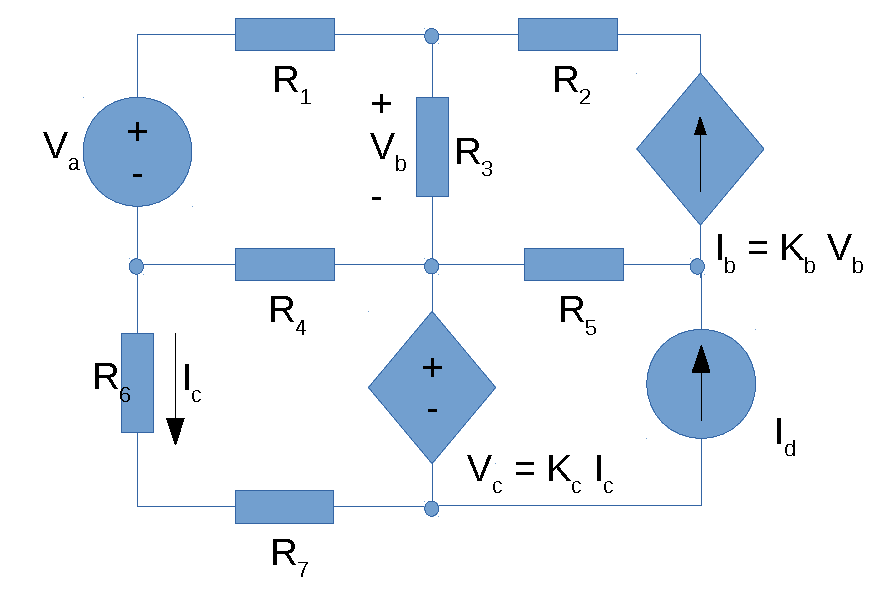
\includegraphics[width=0.4\linewidth]{circuit.pdf}
\caption{Circuit to be analyzed in the laboratory assignment.}
\label{fig:rc}
\end{figure}





\section{Theoretical Analysis}
\label{sec:analysis}

\paragraph{} The values used in both analysis are the following:

$R_1$ = 1.00781211614 $k\Omega$
$R_2$ = 2.00311223204 $k\Omega$
$R_3$ = 3.04503555589 $k\Omega$
$R_4$ = 4.17896607062 $k\Omega$
$R_5$ = 3.10615699135 $k\Omega$
$R_6$ = 2.06090154363 $k\Omega$
$R_7$ = 1.00634569025 $k\Omega$
$V_s$ = 5.04864033546 V
$C$ = 1.02502620056 mA
$K_b$ = 7.05958243797 mS
$K_c$ = 8.03913881798 $m\Omega$

\subsection{Analysis for t<0}

\paragraph{} For t<0 we can see that we are working in the steady state, given that in that time interval $v_S$ = $V_S$. In a DC circuit, the capacitor charges up to it's full capacity, blocking the flow of electricity. Taking 
this into account we can replace the capacitor with an open circuit. With this information, and knowing that the the tension in $V_4$, since it is connected to ground, we can obtain the following equations.

\begin{equation}
\begin{bmatrix}
	-1	&	0	&	0	&	0	&	0	&	0	&	0 \\
	G_1	&	-G_1 - G_2 - G_3	&	G_2	&	G_3	&	0	&	0	&	0 \\
	0	&	-K_b - G_2	&	G_2	&	K_b	&	0	&	0	&	0 \\
	G_1	&	-G_1	&	0	&	-G_4	&	0	&	-G_6	&	0 \\
	0	&	0	&	0	&	0	&	0	&	G_6 + G_7	&	-G_7 \\
	0	&	0	&	0	&	-1	&	0	&	-G_6 *	K_d	&	1 \\
	0	&	G_3	&	0	&	-G_3 - G_4 - G_5	&	G_5	&	-G_6	&	0
\end{bmatrix}
\times
\begin{bmatrix}
	V_1 \\
	V_2 \\
	V_3 \\
	V_5 \\
	V_6 \\
	V_7 \\
	V_8
\end{bmatrix}
=
\begin{bmatrix}
	-V_s \\
	0 \\
	0 \\
	0 \\
	0 \\
	0 \\
	0
	\label{m:1}
\end{bmatrix}
\end{equation}

After solving them with the Octave sofware, we obtained the following results:

[INSERIR TABELA]

%\begin{table}[hbt!]
  %\centering
  %\begin{tabular}{|l|r|}
    %\hline    
 %   {\bf Name} & {\bf Value [mA]} \\ \hline
    %$I_{a}$ & -0.186554\\ \hline
$I_{b}$ & -0.195655\\ \hline
$I_{c}$ & 0.983196\\ \hline
$I_{d}$ & 1.025026\\ \hline

  %\end{tabular}
  %\caption{Mesh currents expressed in mA}
  %\label{tab:op}
%\end{table}

\subsection{Equivalent Resistance}

\paragraph{}In order to determine the equivalent resistance we need to determine $V_X$, this is, the difference between $V_6$ - $V_8$. This is made to ensure that the voltage in the capacitor is continuous.

Making use of the matrix below:

\begin{equation}
\begin{bmatrix}
	-1	&	0	&	0	&	0	&	0	&	0	&	0 \\
	G_1	&	-G_1 - G_2 - G_3	&	G_2	&	G_3	&	0	&	0	&	0 \\
	0	&	-K_b - G_2	&	G_2	&	K_b	&	0	&	0	&	0 \\
	G_1	&	-G_1	&	0	&	-G_4	&	0	&	-G_6	&	0 \\
	0	&	0	&	0	&	0	&	0	&	G_6 + G_7	&	-G_7 \\
	0	&	0	&	0	&	-1	&	0	&	-G_6 *	K_d	&	1 \\
	0	&	0	&	0	&	0	&	-1	&	0	&	1
\end{bmatrix}
\times
\begin{bmatrix}
	V_1 \\
	V_2 \\
	V_3 \\
	V_5 \\
	V_6 \\
	V_7 \\
	V_8
\end{bmatrix}
=
\begin{bmatrix}
	0 \\
	0 \\
	0 \\
	0 \\
	0 \\
	0 \\
	-V_x
	\label{m:1}
\end{bmatrix}
\end{equation}

And knowing that:

\begin{equation}
	V_x = V_6 - V_8
\end{equation}

\begin{equation}
	I_x = \frac{V_6 - V_5}{R_5} + \frac{V_3 - V_2}{R_2}
\end{equation}

\begin{equation}
	R_eq = \frac{V_x}{I_x}
\end{equation}

\begin{equation}
	\tau = R_eq * C
\end{equation}

We can obtain the following values:

[INSERIR TABELA]

\subsection{Natural Solution}

\paragraph{} The natural solution doesn't take into account idependent power sources. Using $V_x$ as the initial condition the natural solution can be obtained with the following equation

\begin{equation}
	V_{6n}(t) = V_x e^{(-\frac{t}{\tau})}
\end{equation}

After computing this data on Octave, we can plot the results of the interval [0, 20]ms.

\begin{figure}[!h]
	\centering
	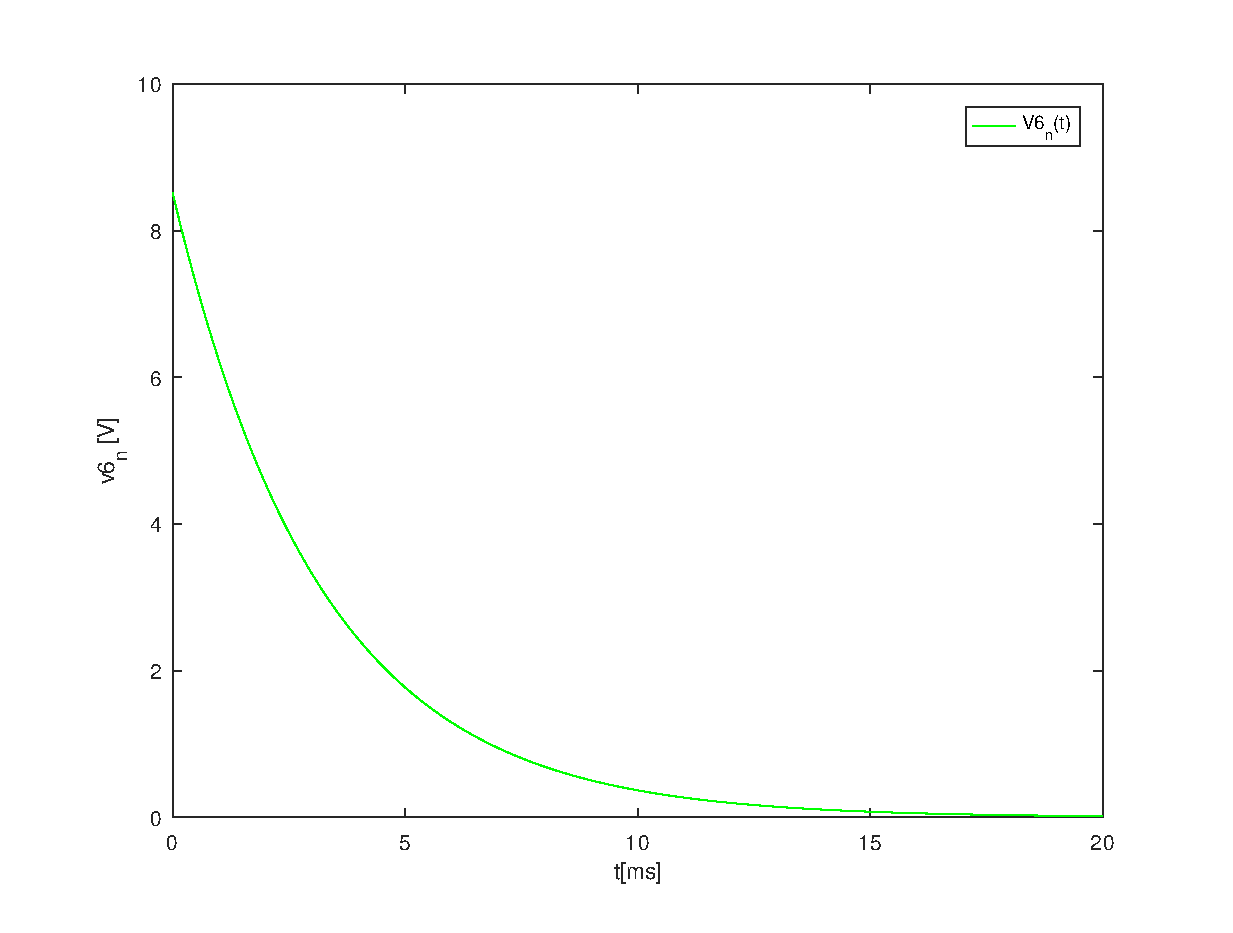
\includegraphics[width=0.7\linewidth]{natural.eps}
	\caption{Natural solution for t € [0, 20]}
\end{figure}

\subsection{Forced Solution}

\paragraph{} In order to obtain the forced solution we must be able to solve the following equation.  

\begin{equation}
\begin{bmatrix}
	-1	&	0	&	0	&	0	&	0	&	0	&	0 \\
	G_1	&	-G_1 - G_2 - G_3	&	G_2	&	G_3	&	0	&	0	&	0 \\
	0	&	-K_b - G_2	&	G_2	&	K_b	&	0	&	0	&	0 \\
	G_1	&	-G_1	&	0	&	-G_4	&	0	&	-G_6	&	0 \\
	0	&	0	&	0	&	0	&	0	&	G_6 + G_7	&	-G_7 \\
	0	&	0	&	0	&	-1	&	0	&	-G_6 *	K_d	&	1 \\
	0	&	G_3	&	0	&	-G_3 - G_4 - G_5	&	G_5 - jwC	&	-G_6	&	jwc
\end{bmatrix}
\times
\begin{bmatrix}
	V_1 \\
	V_2 \\
	V_3 \\
	V_5 \\
	V_6 \\
	V_7 \\
	V_8
\end{bmatrix}
=
\begin{bmatrix}
	-j \\
	0 \\
	0 \\
	0 \\
	0 \\
	0 \\
	0
	\label{m:1}
\end{bmatrix}
\end{equation}

From which we obtain the following values:

\begin{table}[h]
  \centering
  \begin{tabular}{|l|r|r|}
    \hline    
    {\bf Name} & {\bf Complex Amplitude [V]} & {\bf Phase [Degrees]}\\ \hline
    $V_{1}$ & 1.000000 & -90.000000\\ \hline
$V_{2}$ & 0.947229 & -90.000000\\ \hline
$V_{3}$ & 0.832203 & -90.000000\\ \hline
$V_{5}$ & 0.955091 & -90.000000\\ \hline
$V_{6}$ & 0.551847 & 98.938374\\ \hline
$V_{7}$ & 0.360640 & 90.000000\\ \hline
$V_{8}$ & 0.549553 & 90.000000\\ \hline 
  \end{tabular}
  \caption{Nodal analysis for phasor voltage in forced state.}
  \label{tab:phasor}
\end{table}

\subsection{Final Total Solution}

\paragraph{} The final total solution is obtained by superimposing both natural and forced responses:

\begin{equation}
	V_6(t) = V_{6f}(t) + V_{6n}(t)
\end{equation}

We can see the plot of $V_s(t)$ and $V_6(t)$ from -5ms to 20ms [Observações].

\subsection{Frequency Response}

We can see that for low frequencies (<1Hz) every voltage is in phase. The capacitor is given enough time to charge up to the same voltage 
as the voltage source.

\begin{figure}[!h]
	\centering
	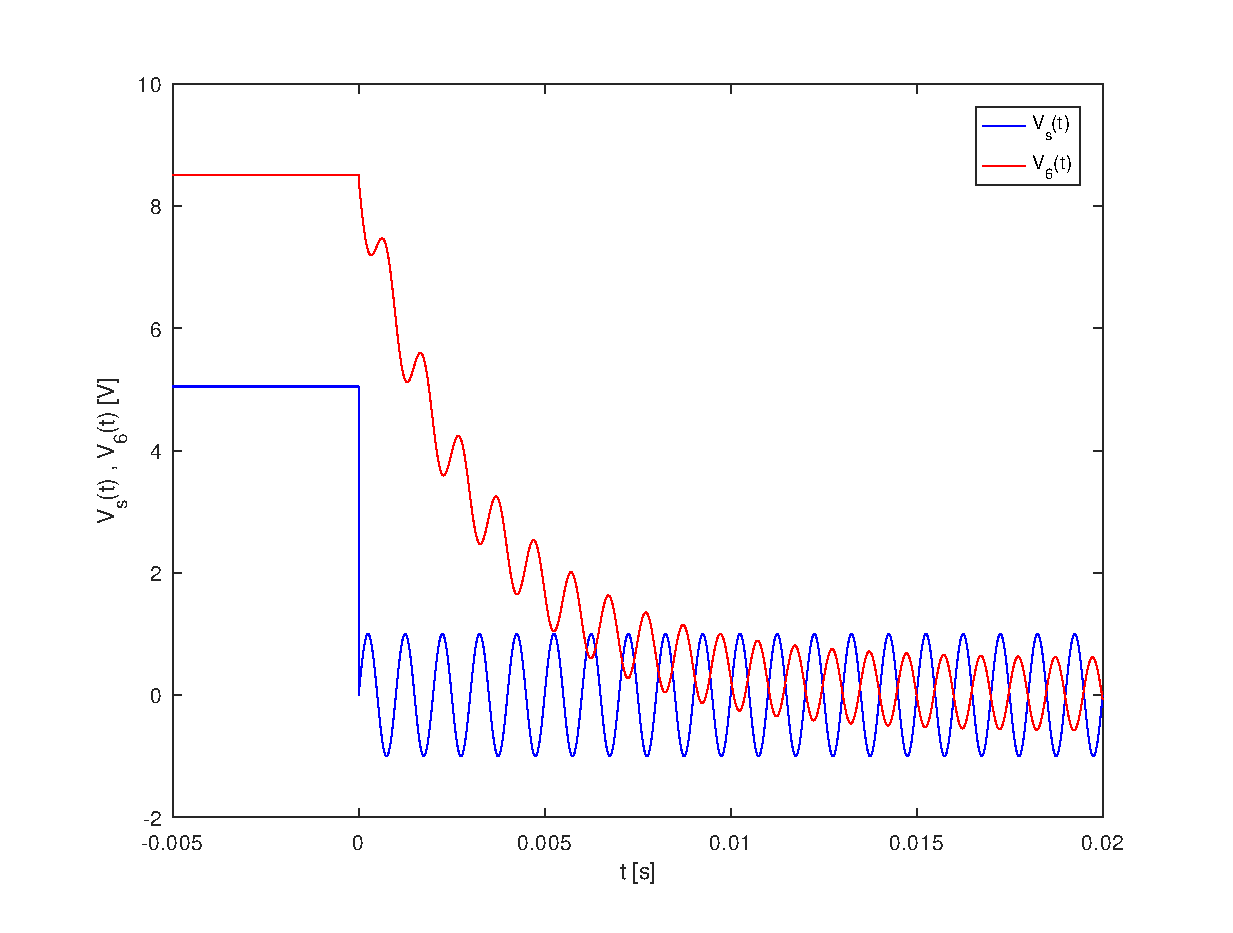
\includegraphics[width=0.7\linewidth]{total.eps}
	\caption{Total solution for $V_6$ and $V_s$}
\end{figure}

\begin{figure}[!h]
	\centering
	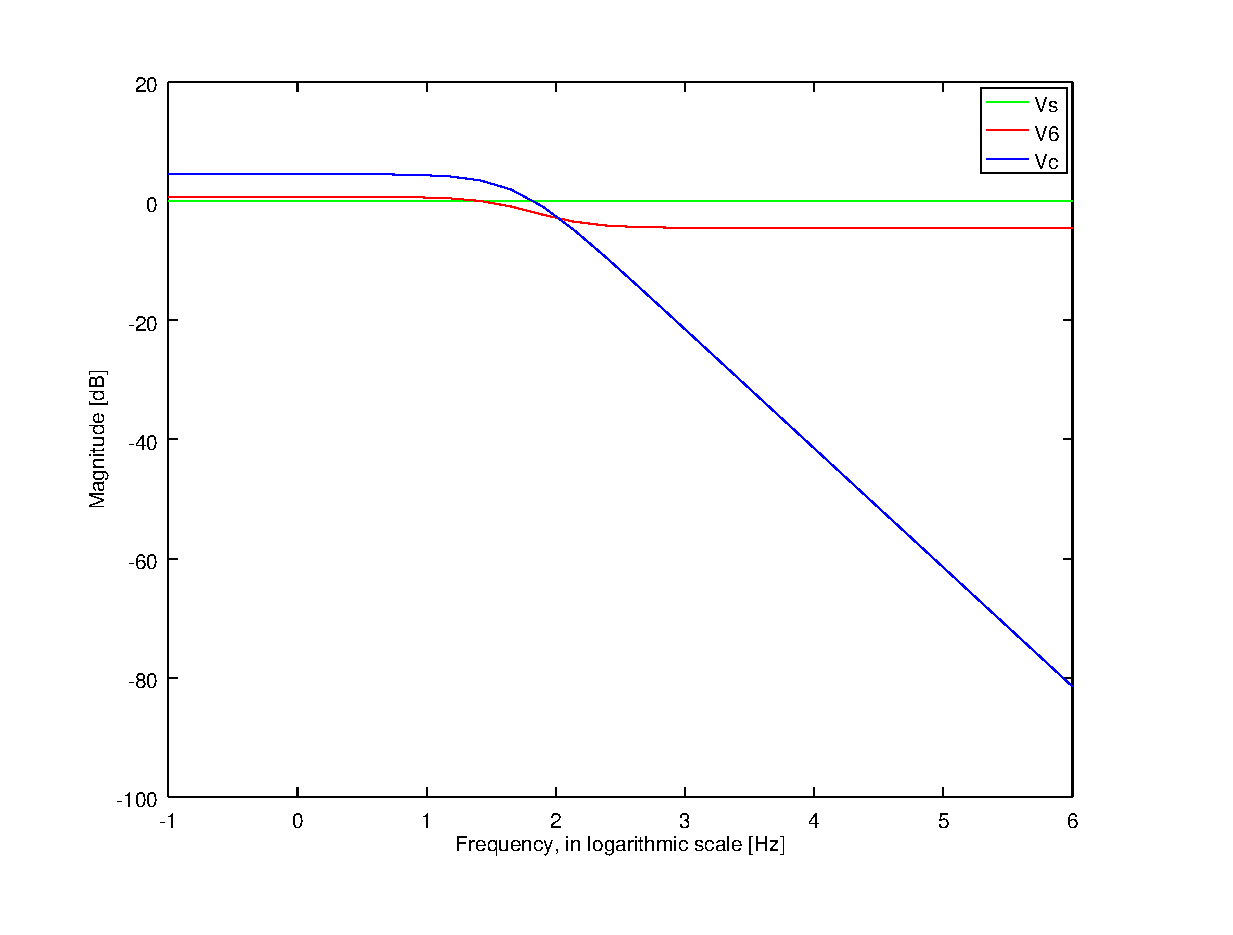
\includegraphics[width=0.7\linewidth]{magnitude.eps}
	\caption{Variation of frequency of $V_s$, $V_6$ and $V_c$ voltage magnitudes}
\end{figure}

\begin{figure}[!h]
	\centering
	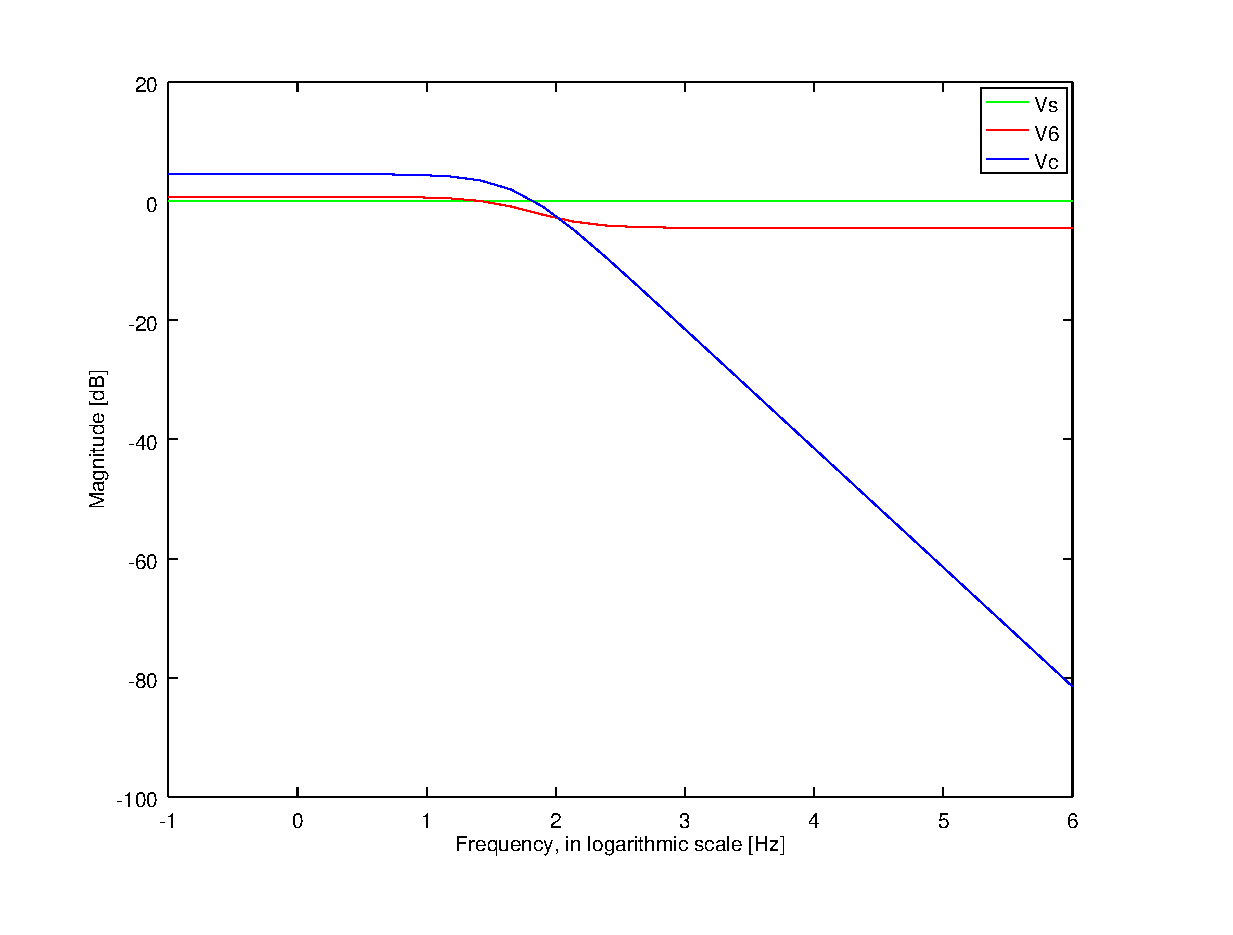
\includegraphics[width=0.7\linewidth]{magnitude.eps}
	\caption{Variation of frequency of $V_s$, $V_6$ and $V_c$ voltage phases}
\end{figure}





%\section{Simulation Analysis}
\label{sec:simulation}

In this section, the circuit shown in Figure~\ref{fig:rc} is simulated with the use of NGSpice. Using the operating point analysis for both $t<0~s$ and $t=0~s$, we determine the initial conditions needed for the transient analysis, which in turn simulates the circuit's total response.
Because of the use of NGSpice for this simulation, there was a need to create a "dummy" voltage source, between nodes 7 and 8, that provided $0~V$ to the circuit (thus not changing the behavior of the original circuit). Because this is just a technical issue that does not affect the original circuit, the one shown in Figure~\ref{fig:rc} can be used for illustrative purposes.


\subsection{Operating Point Analysis}

Table~\ref{tab:op} shows the simulated operating point results for $t<0~s$, where it's assumed that no current flows through the capacitor (open circuit).
Table~\ref{tab:op2} shows the simulated operating point results for $t=0~s$, where $V_S$ is short-circuited and the capacitor is replaced with a voltage source $V_x = V(6) - V(8)$ (with $V(6)$ and $V(8)$ as obtained in Table~\ref{tab:op}.


\begin{table}[h]
	\parbox{.45\linewidth}{
  \centering
  \begin{tabular}{|l|r|}
    \hline    
    {\bf Name} & {\bf Value [A or V]} \\ \hline
    v(1) & 5.048640e+00\\ \hline
v(2) & 4.860629e+00\\ \hline
v(3) & 4.468710e+00\\ \hline
v(4) & 4.888344e+00\\ \hline
v(5) & 8.679973e+00\\ \hline
v(6) & -2.02627e+00\\ \hline
v(7) & -3.01571e+00\\ \hline
v(8) & -3.01571e+00\\ \hline

  \end{tabular}
  \caption{Operating point data for $t<0~s$. A variable preceded by @ is of type Current and is expressed in Ampere; other variables are of type Voltage and are expressed in Volt.}
  \label{tab:op}
}
\hfill
	\parbox{.45\linewidth}{
  \centering
  \begin{tabular}{|l|r|}
    \hline    
    {\bf Name} & {\bf Value [A or V]} \\ \hline
    v(1) & 5.048640e+00\\ \hline
v(2) & 4.860629e+00\\ \hline
v(3) & 4.468710e+00\\ \hline
v(4) & 4.888344e+00\\ \hline
v(5) & 8.679973e+00\\ \hline
v(6) & -2.02627e+00\\ \hline
v(7) & -3.01571e+00\\ \hline
v(8) & -3.01571e+00\\ \hline

  \end{tabular}
  \caption{Operating point data for $t=0~s$. A variable preceded by @ is of type Current and is expressed in Ampere; other variables are of type Voltage and are expressed in Volt.}
  \label{tab:op2}
}	
\end{table}
            

\par Compared to the theoretical analysis results, one notices that the simulated data matches almost perfectly the theoretical values. This is expected, as the circuits being simulated in both scenarios are exclusively composed by linear components. Moreover, the slight discrepancies (of the order of $1e-15$) can be associated to the precision of ngspice and to some approximations made by octave because of the precision of the floating point used.

\newpage
\subsection{Transient Analysis}

\subsubsection{Natural Response}

Figure~\ref{fig:trans} shows the plot of the simulated transient analysis results in the interval $[0, 20]~ms$, using the boundary conditions of $V(6)$ and $V(8)$ as determined before. 
Once again, the simulation data matches with the theoretical natural response prediction, and one can clearly see the negative exponential behavior of $V(6)$, as was expected.

\begin{figure}[h] \centering
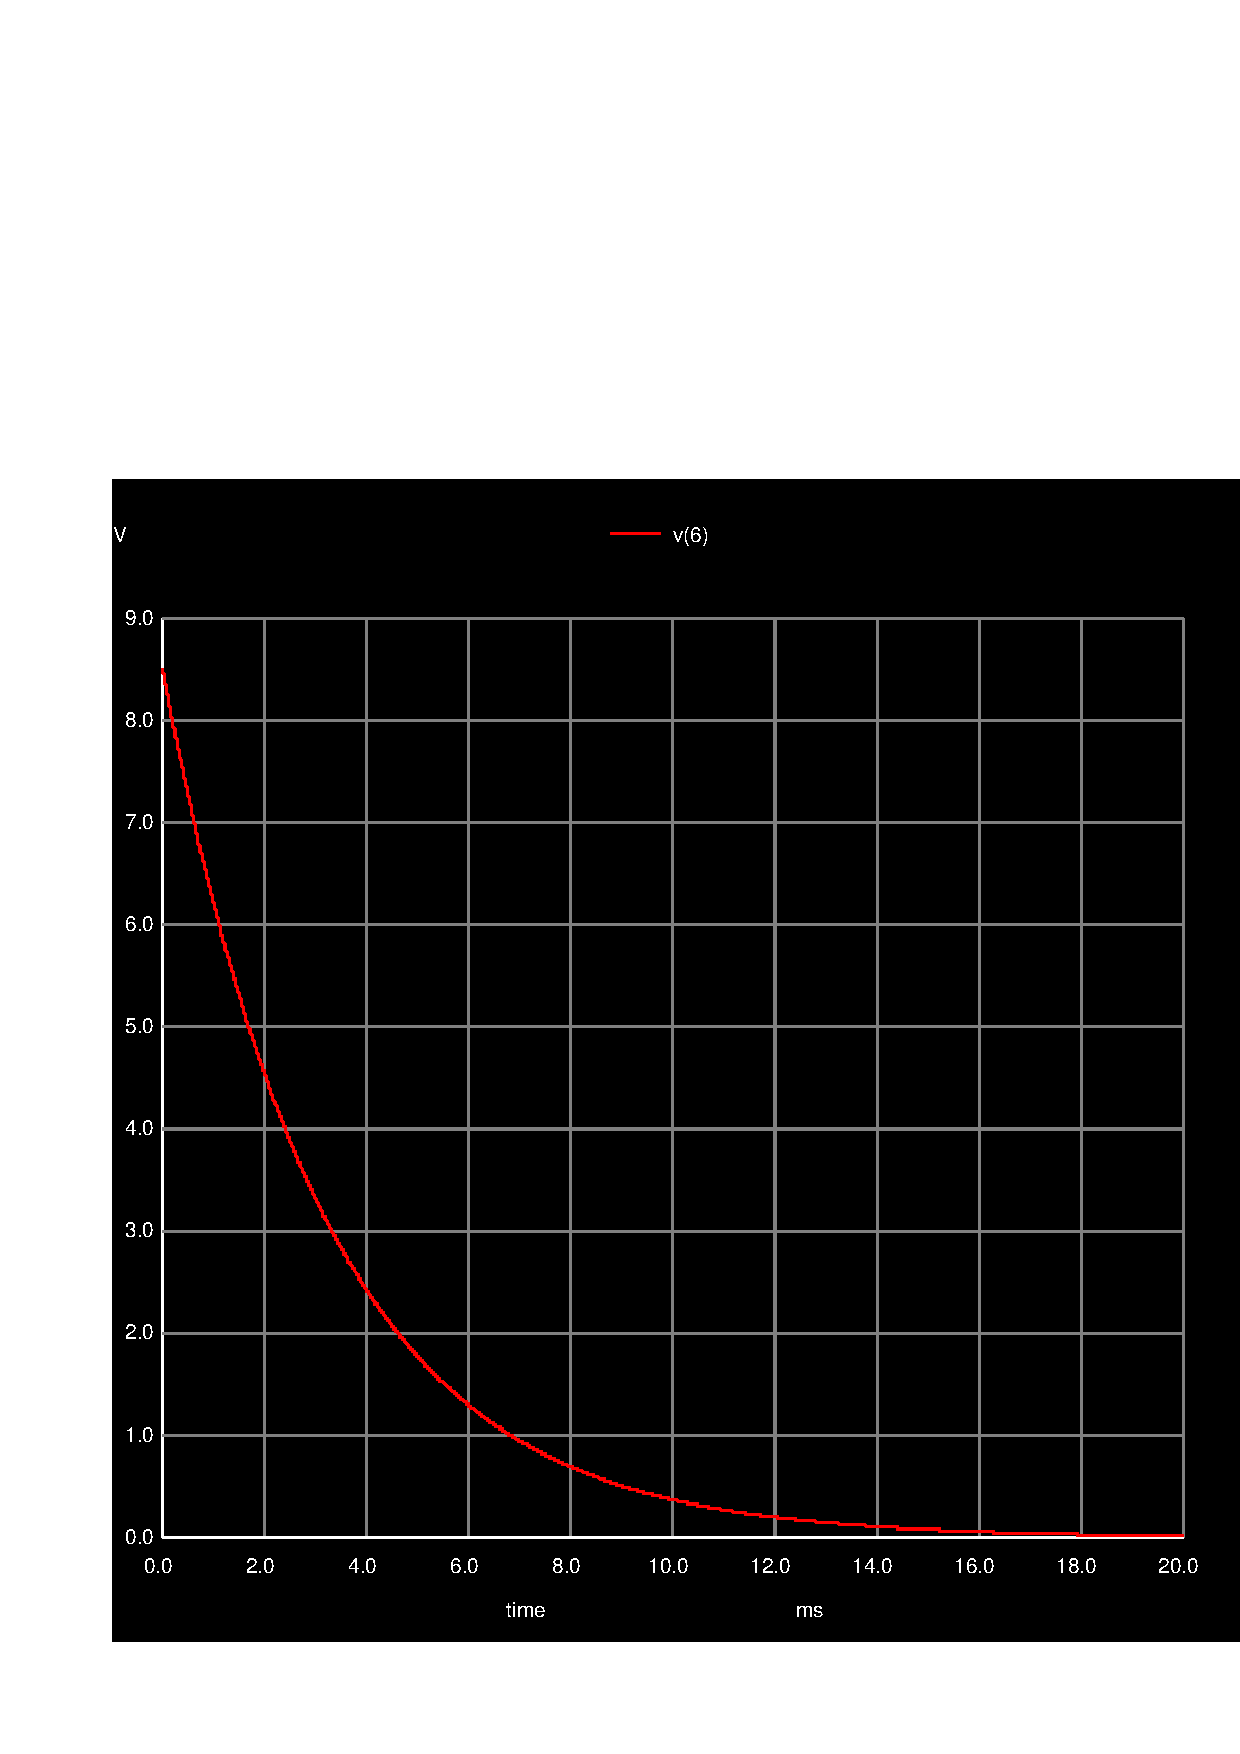
\includegraphics[width=0.6\linewidth]{natural.pdf}
\caption{Natural response of $V_{6}$ in the interval $[0, 20]~ms$.}
\label{fig:trans}
\end{figure}

\newpage

\subsubsection{Total Response}

Figure~\ref{fig:totalsim} shows the plot of the simulated transient analysis results in the interval $[0, 20]~ms$, by using $V_S(t)$ as given in Figure~\ref{fig:rc} and $f = 1~kHz$. 
Once again, the simulation data matches with the theoretical total response prediction, as was expected.
                                    

\begin{figure}[h] \centering
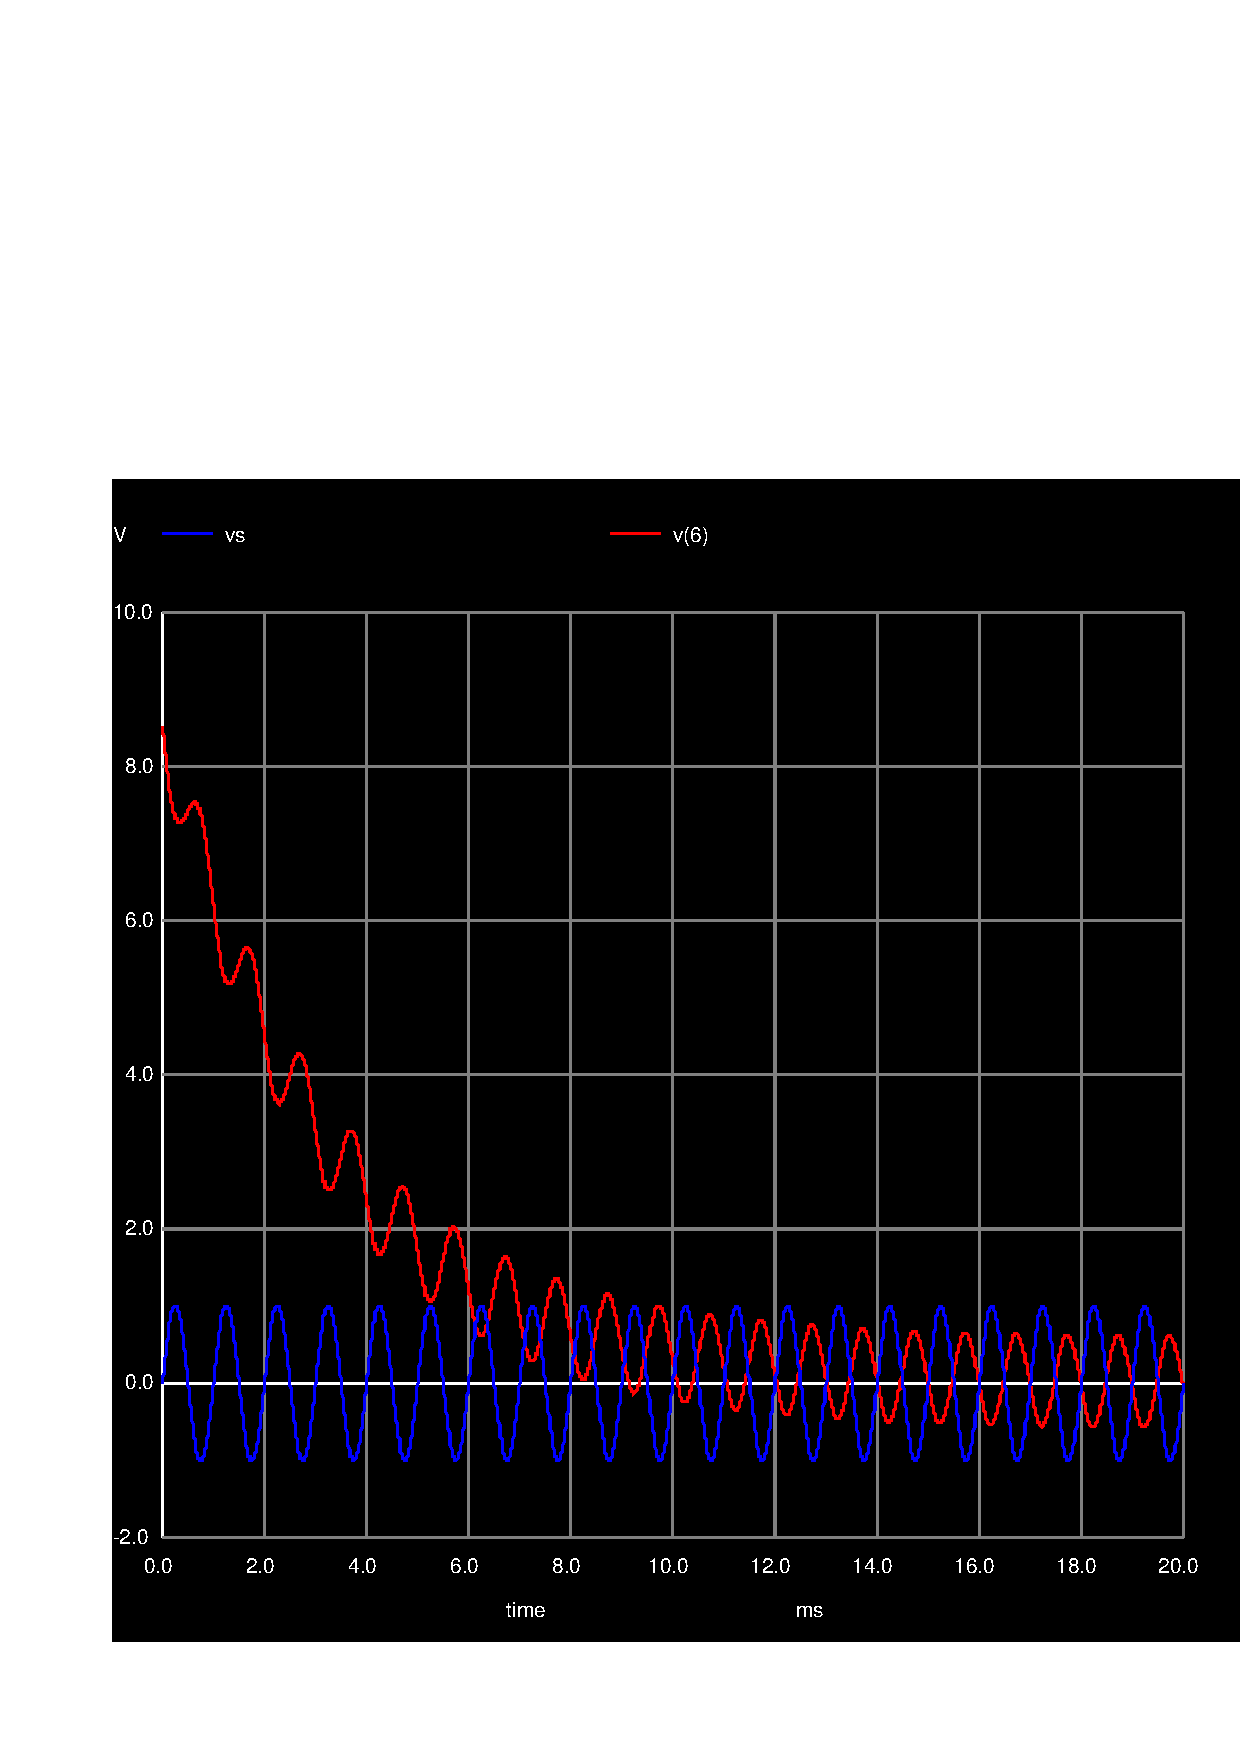
\includegraphics[width=0.6\linewidth]{total.pdf}
\caption{Total response of $V_{6}$ and $V_S$ in the interval $[0, 20]~ms$.}
\label{fig:totalsim}
\end{figure}

\newpage

\subsection{Frequency Analysis}

In this section, the frequency response in node 6 is simulated, with the frequency in logscale, magnitude in $dB$ and phase in $degrees$, for the frequency range of $0.1~Hz$ to $1~MHz$.


\subsubsection{Magnitude Response}

Figure~\ref{fig:magsim} shows the magnitude of the frequency response for the circuit under analysis. Compared to the theoretical analysis results, one notices a clear match between plots. Thus, the reasons for how $V(6)$ and $V_S$ differ from each other are the same as explained in the theoretical analysis above.

\begin{figure}[h] \centering
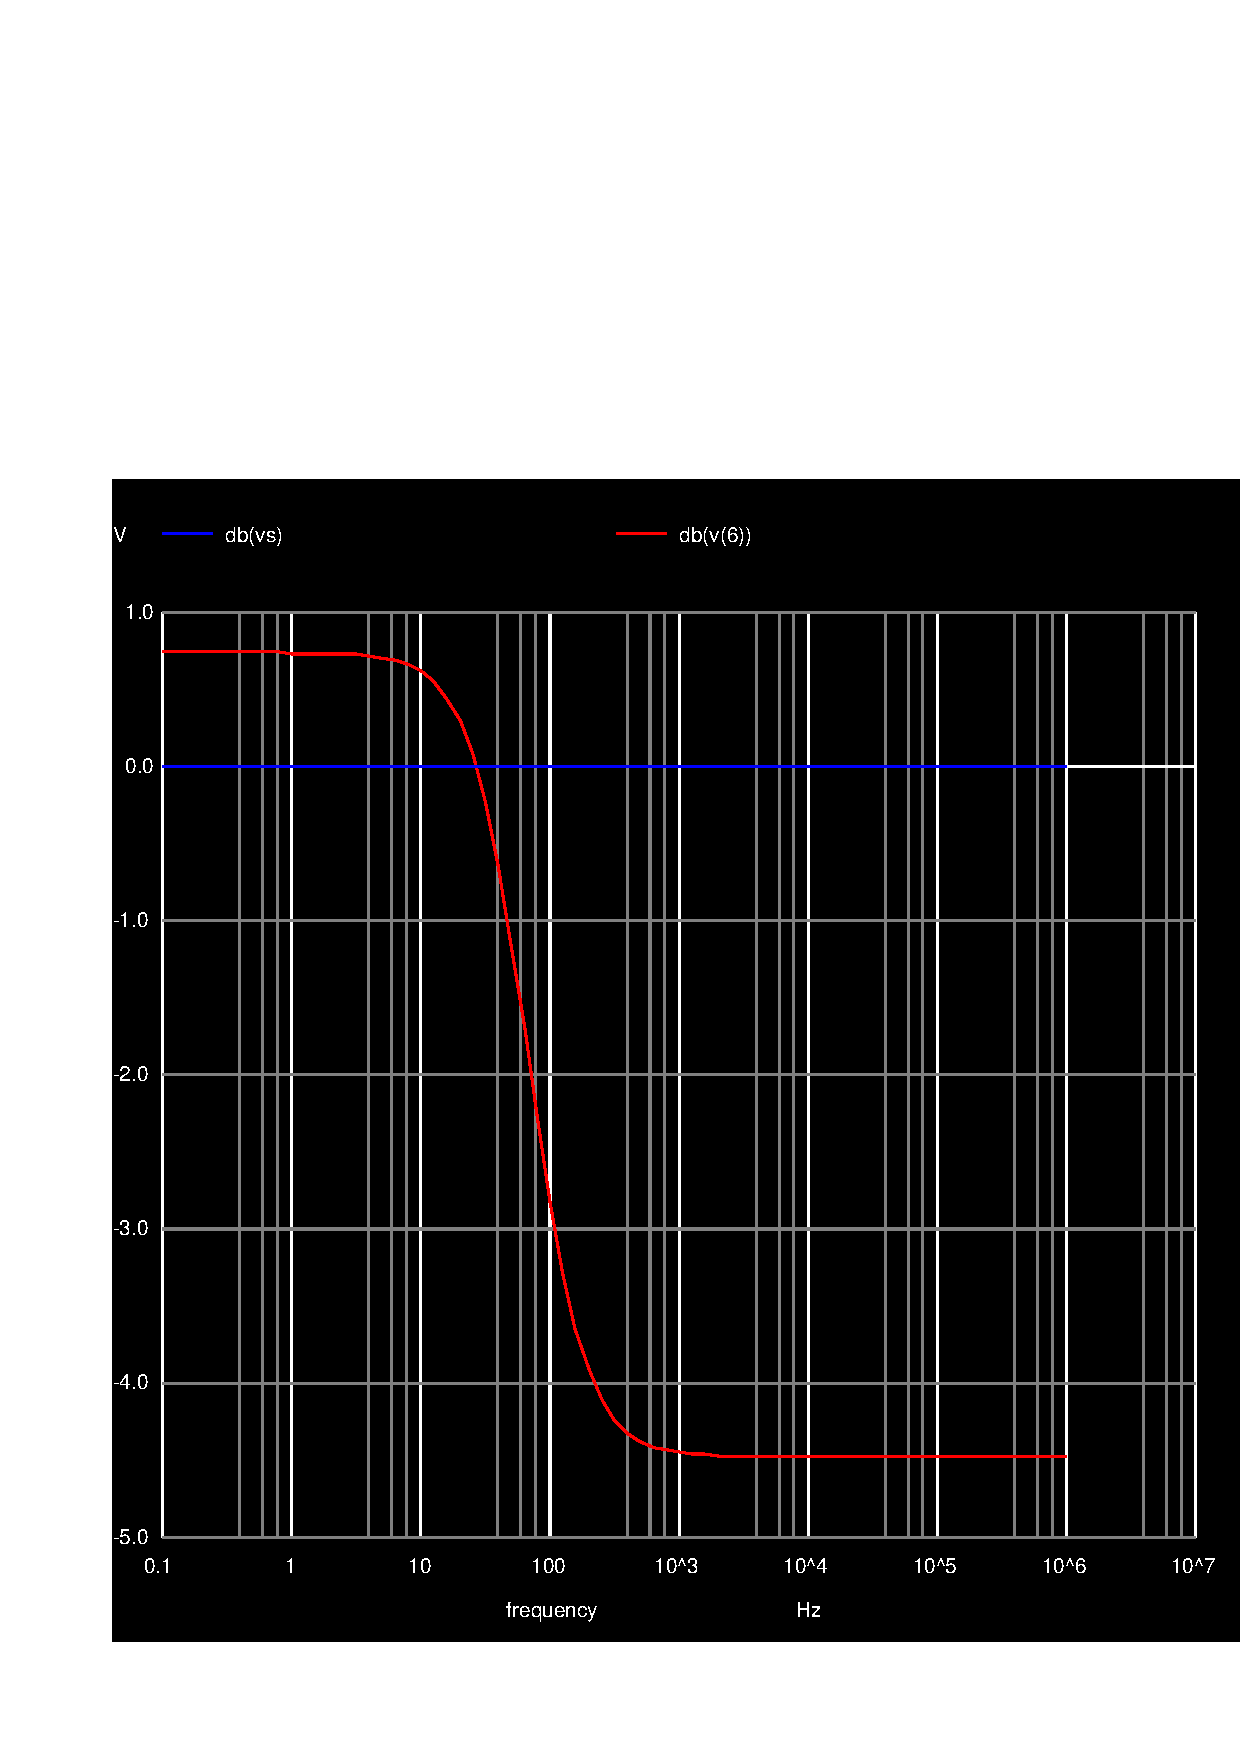
\includegraphics[width=0.6\linewidth]{magnitude.pdf}
	\caption{Magnitude of frequency response of $V(6)$ and $V_S$ plot.}
\label{fig:magsim}
\end{figure}

\newpage

\subsubsection{Phase Response}

Figure~\ref{fig:phasesim} shows the magnitude of the frequency response for the circuit under analysis. Compared to the theoretical analysis results, one notices a clear match between plots. Thus, the reasons for how $V(6)$ and $V_S$ differ from each other are the same as explained in the theoretical analysis above.

\begin{figure}[h] \centering
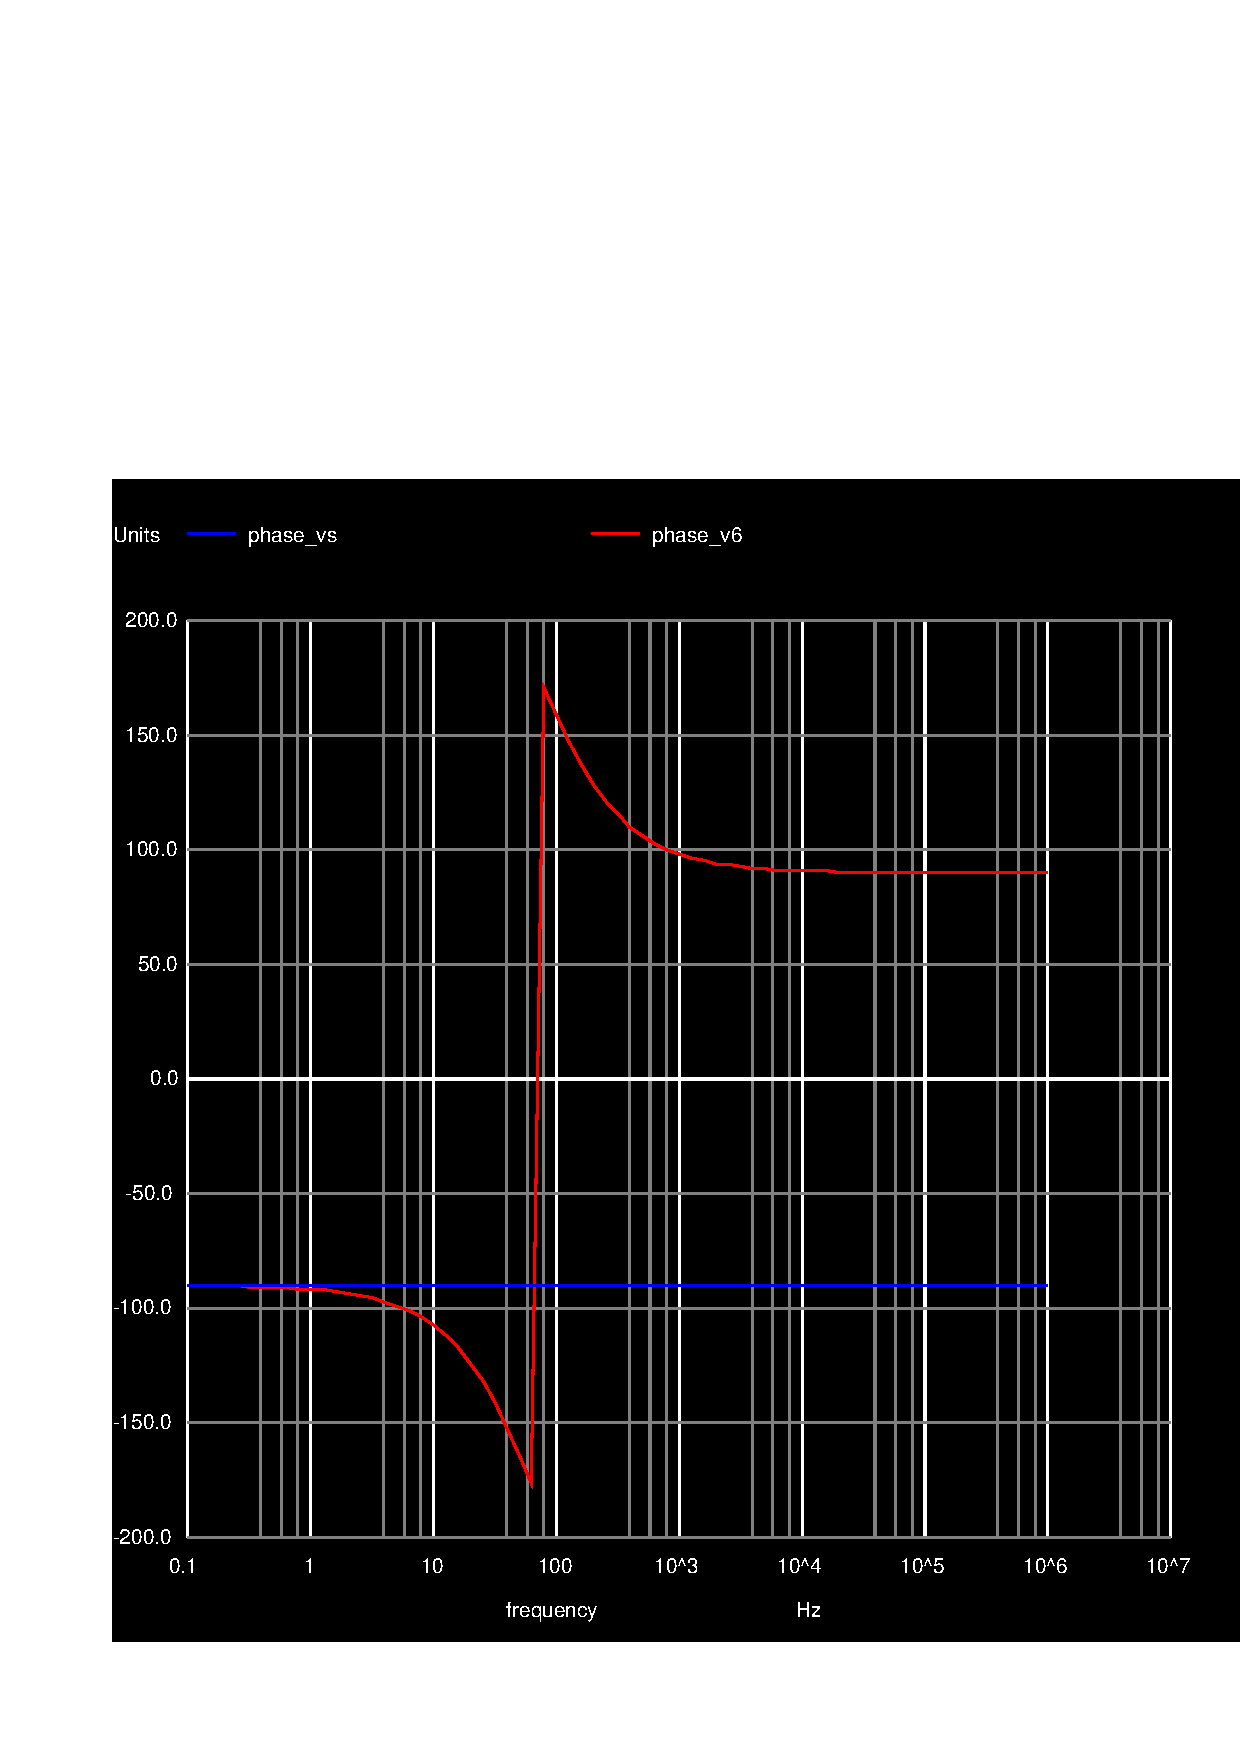
\includegraphics[width=0.6\linewidth]{phase.pdf}
	\caption{Phase response of $V(6)$ and $V_S$ plot.}
\label{fig:phasesim}
\end{figure}



%\section{Conclusion}
\label{sec:conclusion}

\paragraph{} In this laboratory assignment the objective of creating and analysing an Audio Amplifier has been achieved with success. 
We have performed theoreticall and simulation analysis, using the Octave for the former and Ngspice for the latter.

\paragraph{} We found some discrepancies between both sets of results, which can be atributed, among other things, the fact that the circuit 
does not start from equilibrium. The fact that the impedance was high made this more evident. While these discrepancies are not ideal, specially 
for real world aplications, they can be expected and were mitigated.

\paragraph{} The table bellow has the Theoretical and Simulation results, allowing for it's comparison.

\begin{table}[!h]
  \centering
  \begin{tabular}{c c c c}
    \hline    
    {\bf Theoretical} & {\bf Value} & {\bf Simulation} & {\bf Value}\\ \hline
    Frequency response and impedances &  &  &  \\ \hline
$Gain$ & 100.643363 & Gain & 99.7361\\ \hline
$Gain(dB)$ & 40.055703 dB & Gain(dB) & 39.977 dB\\ \hline
$LowerCut-offFreq$ & 723.431560 Hz & Lower cut-off freq & 403.611 Hz\\ \hline
$UpperCut-offFreq$ & 1446.863119 Hz & Upper cut-off freq & 2386.17 Hz\\ \hline
$CentralFreq$ & 1023.086723 Hz & Central freq & 981.37 Hz\\ \hline
$Z_{in} Modulus$ & 1234.241962 Ohm & Zin modulus & 1.23431 kOhm\\ \hline
$Z_{in} Phase$ & -35.883164 Degrees & Zin phase & -35.8894 Degrees\\ \hline
$Z_{out} Modulus$ & 822.637497 Ohm & Zout modulus & 0.826194 kOhm\\ \hline
$Z_{out} Phase$ & -34.650304 Degrees & Zout phase & -34.3981 Degrees\\ \hline
$Cost$ & 13626.952040 & Cost & 1.362695e+04\\ \hline
$Merit$ & 3.092445*$10^{-6}$ & Merit & 3.883972e-06\\ \hline
 
  \end{tabular}
  \caption{Comparison of the theoretical and simulated data results, regarding the operating point, frequency response and impedances.}
  \label{tab:comp}
\end{table}

\paragraph{} We also believe that, given the satisfactory results obtained by us, the model used could be applied in a real life Audio Amplifier.

\paragraph{} Finally, this assignment allowed us to gain some further knowledge in the application of the subjects topics.








%\cleardoublepage

% ----------------------------------------------------------------------
%  Bibliography
% ----------------------------------------------------------------------
%\addcontentsline{toc}{section}{\bibname}
%\bibliographystyle{abbrvunsrtnat} % <<<<< SELECT IF USING REFERENCES BY NUMBER (CITATION ORDER)
%\bibliography{../../../BIBfile.bib}

% ----------------------------------------------------------------------
\end{document}
% ----------------------------------------------------------------------
